\documentclass[11pt,letterpaper]{article}

% \usepackage{epstopdf}% To incorporate .eps illustrations using PDFLaTeX, etc.
% \usepackage[caption=false]{subfig}% Support for small, `sub' figures and tables
%\usepackage[nolists,tablesfirst]{endfloat}% To `separate' figures and tables from text if required
%\usepackage[doublespacing]{setspace}% To produce a `double spaced' document if required
%\setlength\parindent{24pt}% To increase paragraph indentation when line spacing is doubled

% \usepackage[longnamesfirst,sort]{natbib}% Citation support using natbib.sty
% \bibpunct[, ]{(}{)}{;}{a}{,}{,}% Citation support using natbib.sty
% \renewcommand\bibfont{\fontsize{10}{12}\selectfont}% To set the list of references in 10 point font using natbib.sty

\usepackage[natbibapa,nodoi]{apacite}% Citation support using apacite.sty. Commands using natbib.sty MUST be deactivated first!
\setlength\bibhang{12pt}% To set the indentation in the list of references using apacite.sty. Commands using natbib.sty MUST be deactivated first!
\renewcommand\bibliographytypesize{\fontsize{10}{12}\selectfont}% To set the list of references in 10 point font using apacite.sty. Commands using natbib.sty MUST be deactivated first!

% \theoremstyle{plain}% Theorem-like structures provided by amsthm.sty
% \newtheorem{theorem}{Theorem}[section]
% \newtheorem{lemma}[theorem]{Lemma}
% \newtheorem{corollary}[theorem]{Corollary}
% \newtheorem{proposition}[theorem]{Proposition}

% \theoremstyle{definition}
% \newtheorem{definition}[theorem]{Definition}
% \newtheorem{example}[theorem]{Example}

% \theoremstyle{remark}
% \newtheorem{remark}{Remark}
% \newtheorem{notation}{Notation}

%%%%%%%%%%%%%%%%%%%%%%%%%%%%%%%%%%%%%%%%%%%%%%%%%%%%%%%%%%%%%%%%%%%%%%%%%
\pagestyle{plain}                                                      %%
% \pagestyle{empty}                                                      %%
%%%%%%%%%% EXACT 1in MARGINS %%%%%%%                                   %%
\setlength{\textwidth}{6.5in}     %%                                   %%
\setlength{\oddsidemargin}{0in}   %% (It is recommended that you       %%
\setlength{\evensidemargin}{0in}  %%  not change these parameters,     %%
\setlength{\textheight}{8.5in}    %%  at the risk of having your       %%
\setlength{\topmargin}{0in}       %%  proposal dismissed on the basis  %%
\setlength{\headheight}{0in}      %%  of incorrect formatting!!!)      %%
\setlength{\headsep}{0in}         %%                                   %%
\setlength{\footskip}{.5in}       %%                                   %%
%%%%%%%%%%%%%%%%%%%%%%%%%%%%%%%%%%%%                                   %%
\newcommand{\required}[1]{\section*{\hfil #1\hfil}}                    %%
% \renewcommand{\refname}{\hfil References Cited\hfil}                 %%
% \renewcommand{\refname}{References Cited\hfil}                       %%
% \bibliographystyle{plain}                                            %%
%%%%%%%%%%%%%%%%%%%%%%%%%%%%%%%%%%%%%%%%%%%%%%%%%%%%%%%%%%%%%%%%%%%%%%%%%

\usepackage[export]{adjustbox}
\usepackage[linesnumbered,ruled,vlined]{algorithm2e}
\usepackage{amsmath}
% \usepackage{amsthm}
\usepackage{amssymb}
\usepackage{amsfonts}
\usepackage{cancel}
\usepackage{caption}
\usepackage{centernot}
\usepackage{comment}
% \usepackage[shortlabels]{enumitem}
\usepackage{empheq}
\newcommand*\widefbox[1]{\fbox{\hspace{2em}#1\hspace{2em}}}
\usepackage{epsfig}
\usepackage{epstopdf}
% \usepackage[letterpaper, top=1.0in, bottom=1.0in, left=1.0in, right=1.0in]{geometry}
\usepackage{graphics}
\usepackage{graphicx}
\graphicspath{{figures/}}
\usepackage{ifpdf}
\usepackage{lastpage}
\usepackage{lipsum}
\usepackage{leftidx}
\usepackage{mathrsfs}
\usepackage{mathtools}
\usepackage{multicol}
\usepackage{multirow}
% \usepackage[square, numbers, comma, sort&compress]{natbib}
\usepackage{nicefrac}
\usepackage{nicematrix}
\usepackage{pgfplots}
\usepackage{ragged2e}
\usepackage{rotating}
\usepackage{stmaryrd}
\usepackage{tabularx}
\usepackage{tikz}
\usepackage{tkz-euclide}
\usepackage{ctable}
\usetikzlibrary{matrix, arrows}
\usepackage{todonotes}
% \usepackage{ulem} // Messes up italics in references
\usepackage{wrapfig}
\usepackage{xcolor}

\usepackage{hyperref}
\hypersetup{
    bookmarks=true,         % show bookmarks bar?
    unicode=false,          % non-Latin characters in Acrobat’s bookmarks
    pdftoolbar=true,        % show Acrobat’s toolbar?
    pdfmenubar=true,        % show Acrobat’s menu?
    pdffitwindow=false,     % window fit to page when opened
    pdfstartview={FitH},    % fits the width of the page to the window
    pdftitle={Inverse Kinematics via Gaussian Mixture Modeling},    % title
    pdfauthor={Aykut C. Satici},     % author
    % pdfsubject={Subject},   % subject of the document
    % pdfcreator={Creator},   % creator of the document
    % pdfproducer={Producer}, % producer of the document
    % pdfkeywords={keyword1, key2, key3}, % list of keywords
    pdfnewwindow=true,      % links in new PDF window
    colorlinks=true,       % false: boxed links; true: colored links
    linkcolor=magenta,          % color of internal links (change box color with linkbordercolor)
    linkbordercolor=orange,
    citecolor=blue,        % color of links to bibliography
    citebordercolor=green,
    filecolor=magenta,      % color of file links
    urlcolor=cyan,           % color of external links
    urlbordercolor=blue,
}


\makeatletter
\newcommand{\rmnum}[1]{\romannumeral #1}
\newcommand{\Rmnum}[1]{\expandafter\@slowromancap\romannumeral #1@}
\makeatother



\newcommand{\bmat}[1]{\begin{bmatrix}#1\end{bmatrix}}
\newcommand{\ubar}[1]{\text{\b{$#1$}}}
\newcommand{\norm}[2]{\|{#1}\|_{{}_{#2}}}
\newcommand{\abs}[1]{\left|{#1}\right|}
\newcommand{\mbf}[1]{\mathbf{#1}}
\newcommand{\mc}[1]{\mathcal{#1}}
\newcommand{\dd}{\operatorname{d}\!}
\newcommand{\muc}[2]{\multicolumn{#1}{c}{#2}}
\newcommand*\Eval[3]{\left.#1\right\rvert_{#2}^{#3}}
\newcommand{\inner}[1]{\left\langle#1\right\rangle}
\newcommand{\pd}[2]{\frac{\partial #1}{\partial #2}}
\newcommand{\pdd}[2]{\frac{\partial^2 #1}{\partial #2^2}}
\newcommand{\el}[2]{\frac{\dd}{\dd t}\pd{\mc{L}}{\dot{#1}} - \pd{\mc{L}}{#1} = #2}
\newcommand{\elk}[2]{\frac{\dd}{\dd t}\pd{\mc{L}}{\dot{#1}_k} - \pd{\mc{L}}{#1_k} = #2_k}
\newcommand{\vectornorm}[1]{\left|\left|#1\right|\right|}
\newcommand{\dom}[1]{\textrm{dom}\;#1}
\newcommand\blfootnote[1]{%
  \begingroup
  \renewcommand\thefootnote{}\footnote{#1}%
  \addtocounter{footnote}{-1}%
  \endgroup
}
\newcommand{\bx}{{\bf x}}
\newcommand{\bu}{{\bf u}}

\newtheorem{defn}{Definition}
\newtheorem{thm}{Theorem}[section]
\newtheorem{lem}[thm]{Lemma}
\newtheorem{prop}{Proposition}[section]
\newtheorem{rem}{Remark}

\DeclareMathOperator{\Tr}{tr}
\newcommand\xdownarrow[1][2ex]{%
   \mathrel{\rotatebox{90}{$\xleftarrow{\rule{#1}{0pt}}$}}
}
\DeclareMathOperator{\End}{End}
\DeclareMathOperator{\Hom}{Hom}
\DeclareMathOperator{\id}{id}
\DeclareMathOperator{\vers}{vers}
\DeclareMathOperator{\trans}{Trans}
\DeclareMathOperator{\rot}{Rot}
\DeclareMathOperator{\rank}{rank}
\DeclareMathOperator{\sinc}{sinc}

\newenvironment{itquote}
  {\begin{quote}\itshape}
  {\end{quote}\ignorespacesafterend}

% \pagenumbering{arabic}

\begin{document}

% \articletype{}% Specify the article type or omit as appropriate

% \title{\.{I}lgin\c{c} Bir Olas{\i}l{\i}k Sorusu}
\section*{
    \begin{center}
        Inverse Kinematics via Gaussian Mixture Modeling
    \end{center}
}

\begin{center}
    Aykut C. Satici\textsuperscript{} \\[0ex]
    July 08, 2021
\end{center}


  
% \vspace{-1mm}
\section{Problem Statement}
%
% \begin{wrapfigure}{r}{0.4\textwidth} %this figure will be at the right
%     \vspace{-5mm}
%     \centering
%     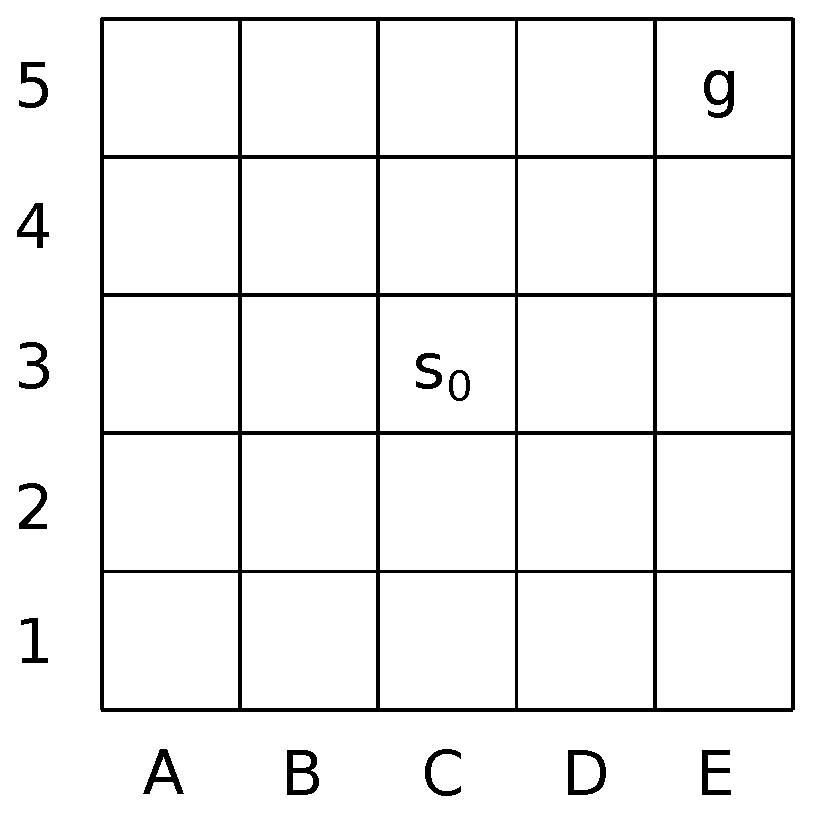
\includegraphics[width=0.25\textwidth]{./figures/drawing.eps}
%     \caption{Schematic of the problem}
%     \label{fig:schematic}
%     \vspace{-5mm}
% \end{wrapfigure}
%
We want to come up with a general procedure that solves the inverse kinematics
problem for redundant manipulators. We will, in particular, work with the planar
three-link articulated robot. We are only interested in the position of its
end-effector. Therefore, the forward kinematics map goes from the joint angles:
$\theta = (\theta_1, \theta_2, \theta_3)$ to $\mathrm{x} = (x,y)$. 
\section{Solution of the Problem}
\label{sec:solution}

The solution will be to utilize a Gaussian Mixture Model (GMM) to represent the
inverse kinematics map. My presentation will closely follow three
sources:~\cite{mclachlan2007algorithm,ghahramani1993solving,xu2017data}.

We assume that the data $\Xi = \left\{ \xi_1, \ldots, \xi_N \right\}$ were
generated independenty by a mixture density:
%
\begin{equation}
    P(\xi_i) = \sum_{j=1}^M \underbrace{P(\omega_j)}_{\pi_j} 
        P(\xi_i \mid \omega_j; \psi_j),
    \label{eq:mixture_density}
\end{equation}
%
where $\{\pi_j\}_j^M$ are the mixture proportions, each component of the mixture
is denoted $\omega_j$ and parametrized by $\psi_j$. The mixture proportions are
to be picked such that \[ \sum_{j=1}^M \pi_j = 1. \] The full set of parameters
of this model are $\pi_j$'s and $\psi_j$'s. We will write $\Psi = (\pi_j,
\psi_j)_j$. When we restrict these probability distributions to be Gaussian, we
will further have $\psi_j = (\mu_j, \Sigma_j)$, where $\mu_j$ is the mean and
$\Sigma_j$ the covariance of the $j^{\textrm{th}}$ Gaussian. The log of the
likelihood of the parameters given the data set is
%
\begin{equation}
    \ell(\Psi \mid \Xi) = \log{ \Pi_{i=1}^N \sum_{j=1}^M P(\xi_i \mid \omega_j; 
    \psi_j) P(\omega_j) } = \sum_{i=1}^N \log{ \sum_{j=1}^M 
    P(\xi_i \mid \omega_j; \psi_j) P(\omega_j). }
    \label{eq:loglike}
\end{equation}
%
We seek to find the parameter vector $\Psi$ that maximizes $\ell(\Psi \mid
\Xi)$. However, this function is not easily maximized numerically because it
involves the log of a sum. Intuitively, it is not easily maximized because for
each data point, there is a ``credit-assignment'' problem, i.e., it is not clear
which component of the mixture generated the data point and thus which
parameters to adjust to fit that data point.

The expectation maximization (EM) algorithm applied to mixtures is an iterative
method for overcoming this credit-assignment problem. The intuition behind it is
that if one had access to a ``hidden'' random variable $z$ that indicated which
data point was generated by which component, then the maximization problem would
decouple into a set of simple maximizations. Mathematically, given $\mc{Z} =
\{z_1, \ldots, z_N \}$ a ``complete-data'' log likelihood function could be
written,
%
\begin{equation}
    \ell_c(\Psi \mid \Xi, \mc{Z}) = \sum_{i=1}^N \sum_{j=1}^M z_{ij} \log{
        P(\xi_i \mid z_i; \Psi)P(z_i; \Psi),
    }
    \label{eq:complete_loglike}
\end{equation}
%
such that it does not involve a log of a summation.

As proven in~\cite{dempster1977maximum}, $\ell(\Psi \mid \Xi)$ can be maximized
by iterating the following two steps,
%
\begin{align}
    \begin{split}
    \text{E-step: } \quad &Q(\Psi \mid \Psi_k) = \mathbb{E}\left[ \ell_c(\Psi \mid \Xi, \mc{Z}) \mid \Xi, \Psi_k \right] \\
    \text{M-step: } \quad &\Psi_{k+1} = \arg \max_\Psi Q(\Psi \mid \Psi_k).
    \end{split}
    \label{eq:EM_alg}
\end{align}
%
The E (Expectation) step computes the expected complete data log likelihood and 
the M (Maximization) step finds the parameters that maximize this likelihood.

\subsection{Mixture of Gaussians}
Let me now specialize to the case where the probability functions above are
Gaussians. For this model, the E-step simplifies to computing $h_{ij} =
\mathbb{E}\left[ z_{ij} \mid \xi_i, \psi_k \right]$, the probability that
Gaussian $j$, as defined by the mean $\hat{\mu}_j$ and covariance matrix
$\hat{\Sigma}_j$ estimated at time step $k$, generated data point $i$:
%
\begin{equation}
    h_{ij}^k = \frac{\abs{\hat{\Sigma}_j^k}^{-\frac{1}{2}} 
    \exp{\left\{-\frac{1}{2}\left( \xi_i - \hat{\mu}_j^k \right)^\top 
    ({\hat{\Sigma}_j^k})^{-1} \left( \xi_i - \hat{\mu}_j^k \right) \right\}}  }
    {\sum_{l=1}^M \abs{\hat{\Sigma}_j^k}^{-\frac{1}{2}} 
    \exp{\left\{-\frac{1}{2}\left( \xi_i - \hat{\mu}_l^k \right)^\top 
    ({\hat{\Sigma}_l^k})^{-1} \left( \xi_i - \hat{\mu}_l^k \right) \right\}} }.
    \label{eq:E-step}
\end{equation}
%
The M-step then involves re-estimating the means and covariances of the
Gaussians along with the mixing proportions using the data set weighted by the
$h_{ij}$:
%
\begin{equation}
    \hat{\mu}_j^{k+1} = \frac{\sum_{i=1}^N h_{ij}^k\xi_i}{\sum_{i=1}^N h_{ij}^k}, \quad
    \hat{\Sigma}_j^{k+1} = \frac{\sum_{i=1}^N h_{ij}^k \left(\xi_i - \hat{\mu}_j^{k+1}\right)
                    \left(\xi_i - \hat{\mu}_j^{k+1}\right)^\top}{\sum_{i=1}^N h_{ij}^k}, \quad
    \pi_j^{k+1} = \frac{1}{N}\sum_{i=1}^N h_{ij}^k.
    \label{eq:M-step}
\end{equation}


\subsection{Supervised Learning}
%
When viewed as supervised learning, each vector $\xi_i$ in the training set is
composed of an ``input'' subvector $\mathrm{x}_i$ and a ``target'' or output
subvector $\theta_i$. Applying the learning algorithm, we obtain an estimate of
the density of the data in this input/output space. This estimate can be used to
approximate a function in the following way:

Given the input vector $\mathrm{x}_i$, we extract all the relevant information
from the joint probability density function (pdf) $P(\mathrm{x}, \theta)$ by
marginalizing to $P(\theta \mid \mathrm{x})$. For a single Gaussian this
conditional density is normal, and by linearity, since $P(\mathrm{x}, \theta)$
is a mixture of Gaussians, so is $P(\theta \mid \mathrm{x})$. In principle, this
conditional density is the final output of the density estimator. That is, given
a particular input, the network returns the complete conditional density of the
output. However, for the purposes of comparison to function approximation
methods and since many applications require a single estimate of the output, I
will outline two possible ways to obtain such an estimate $\hat{\theta}_i$ of
$\theta_i = f(x_i)$.

\bibliographystyle{apacite}
\bibliography{bib/main}

\end{document}
